\hypertarget{part--image-2}{%
\section{Part 3, Image 2}\label{part-1-design-5}}


\centering


\hypertarget{description}{%
	\subsubsection{Description}\label{description}}

\begin{description}
	\item[Image:] xxx
	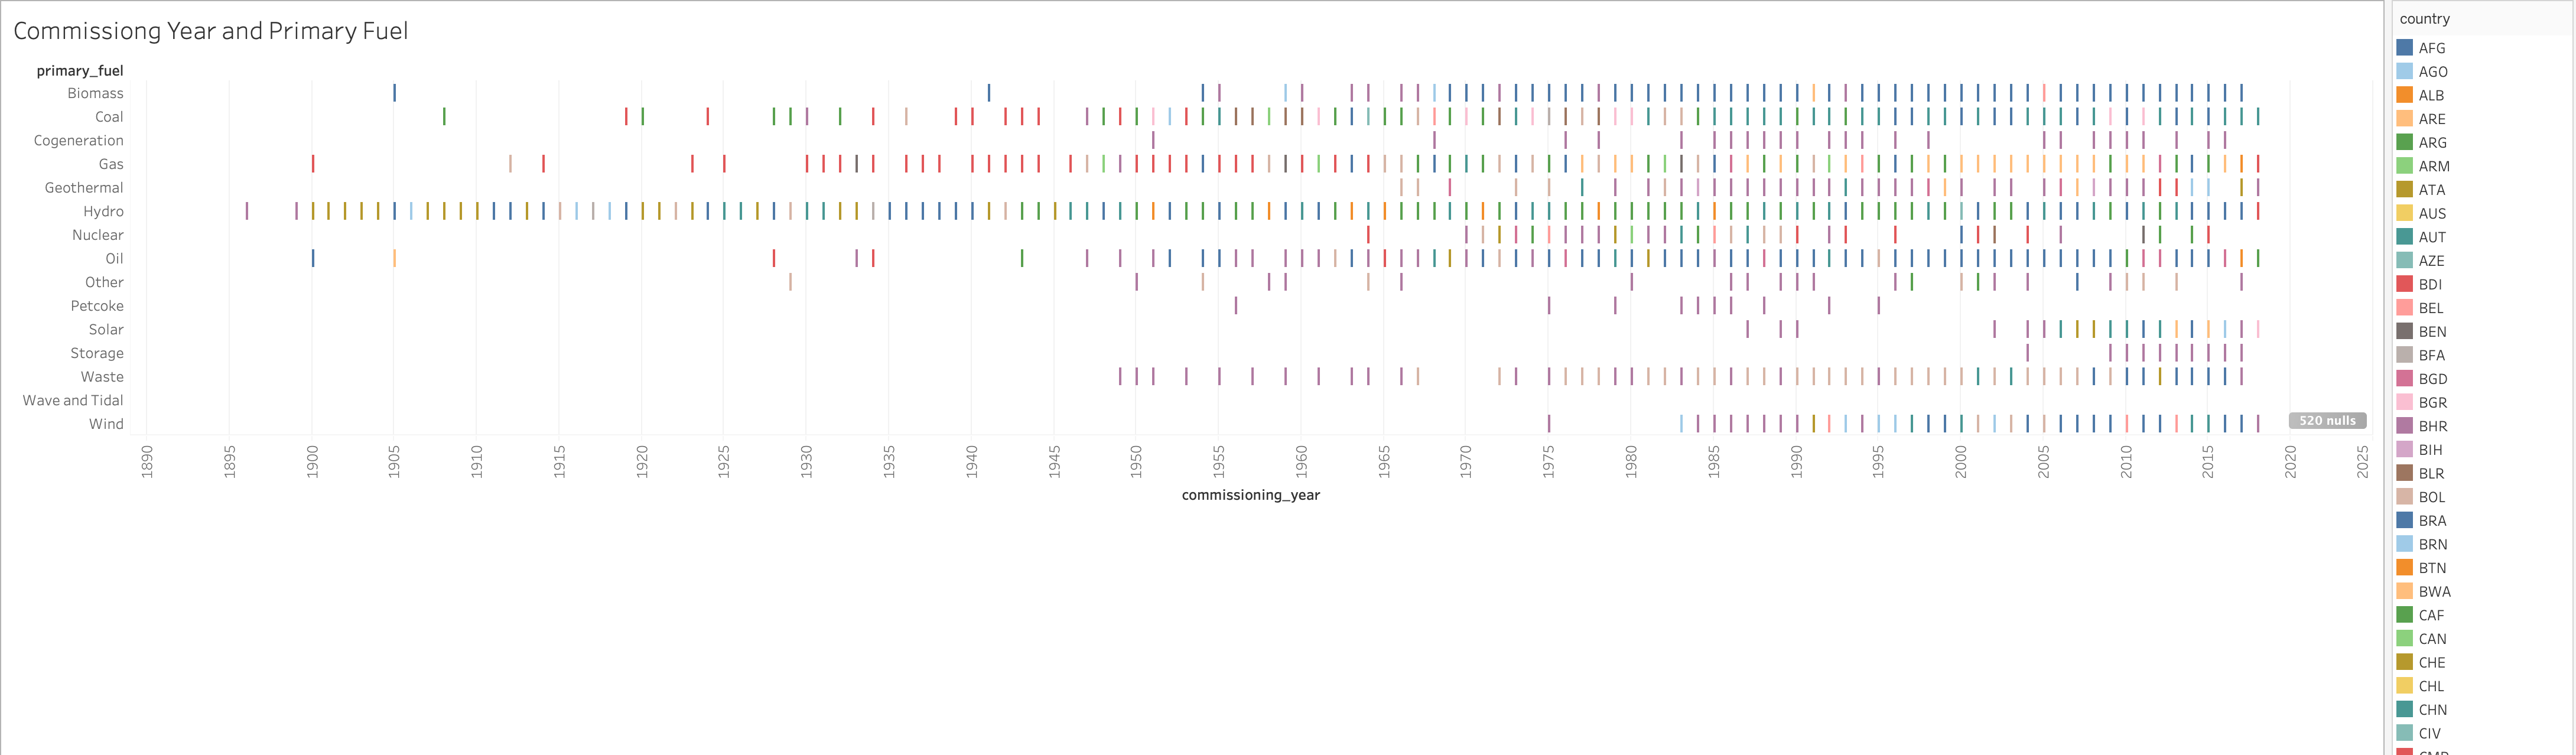
\includegraphics[width=15cm]{Viz1.png}
	\item[Tool:] xxx
	The name of the tool used to generate the image
	\item[Visualization Type:] xxx
	The name/type of the visualization
	\item[Year:] xxx
	1896 - 2018
	\item[Visual Mappings:] xxx
	\begin{itemize}
		\tightlist
		\item[ !!!! Each of the visual mappings, e.g., color is mapped to . . . ,
		opacity is mapped to. . . , - Delete this and leave blank!!!! ] 
	\end{itemize}
	\begin{itemize}
		\tightlist
		\item
		\textbf{mapping 1}: Answer
	\end{itemize}
	
	\begin{itemize}
		\tightlist
		\item
		\textbf{mapping 2}: Answer
	\end{itemize}
	\item[Unique Observation:]
	
\end{description}
